\section{Experiments}
\label{sec:experiments}

\subsection{Experimental Setup}

This section describes the datasets, evaluation metrics, and implementation settings used for the main TAMR-DTI experiments. All main results use the full eight-conformer TAMR-DTI model and five fixed random seeds, $\{42,43,44,45,47\}$. For every run, the best checkpoint is selected by validation AUROC. When a threshold-dependent result uses a tuned operating point, the classification threshold is selected only on the validation split and is then applied unchanged to the held-out test split; such results are reported as Acc(val-thr) and F1(val-thr). Fixed-threshold results, when reported, are denoted Acc@0.5 and F1@0.5.

\subsubsection{Datasets and Data Distribution}

We evaluate TAMR-DTI on four benchmark drug-target interaction (DTI) datasets: BindingDB, BioSNAP, Human, and C. elegans. Each sample consists of a drug SMILES string, a protein sequence, and a binary interaction label. Table~\ref{tab:dataset_overview} reports the aggregate statistics after merging the processed training, validation, and test split files used in this study; the corresponding split-level statistics are moved to Appendix Table~\ref{tab:data_split_appendix}. These processed-split statistics are used throughout the experiments, because they reflect the exact drug-target pairs available to the model after preprocessing.

BindingDB is a public database of experimentally measured protein-ligand binding affinities and drug-target interactions \citep{liu2007bindingdb}. In our processed splits, it is the largest benchmark, with 49,199 labeled interactions, 14,643 drugs, and 2,623 proteins. Its positive rate is 42.02\%, giving a moderate negative-label skew. We use BindingDB to test whether TAMR-DTI can scale to broad chemical and target coverage while remaining robust under non-balanced label distributions.

BioSNAP comes from the Stanford Biomedical Network Dataset Collection and provides curated biomedical network data, including drug-target associations \citep{biosnapnets}. The processed BioSNAP benchmark is medium-sized, with 27,464 interactions, and is nearly class-balanced, with a 50.36\% positive rate. Compared with BindingDB, it offers a different curation source and a more balanced decision setting. We therefore use BioSNAP to evaluate generalization under a network-derived DTI distribution and to support the component analyses in later sections.

The Human benchmark follows the compound-protein interaction dataset introduced with high-confidence negative sample construction \citep{liu2015credible}. It is the smallest benchmark in our study, with 5,997 interactions and a 43.91\% positive rate. Its compact benchmark size and stronger negative skew make it useful for testing model stability when fewer training examples are available and thresholded metrics are more sensitive to class distribution.

The C. elegans benchmark uses the corresponding Caenorhabditis elegans compound-protein interaction data from the same dataset family \citep{liu2015credible}. The processed split contains 7,786 interactions and is exactly balanced in aggregate. Because it represents a non-human model organism, it complements the Human benchmark and tests whether the learned drug and protein representations transfer across organism-specific interaction sources rather than only across larger mixed-source datasets.

\begin{table}[!htbp]
\caption{Dataset statistics used in the main experiments. Counts are computed from the processed training, validation, and test split files used in this study.}
\label{tab:dataset_overview}
\begin{center}
\begin{tabular}{lrrrrrr}
\toprule
Dataset & Drugs & Proteins & Interactions & Positive & Negative & Positive rate \\
\midrule
BindingDB & 14,643 & 2,623 & 49,199 & 20,674 & 28,525 & 42.02\% \\
BioSNAP & 4,505 & 2,181 & 27,464 & 13,830 & 13,634 & 50.36\% \\
Human & 2,726 & 2,001 & 5,997 & 2,633 & 3,364 & 43.91\% \\
C. elegans & 1,767 & 1,876 & 7,786 & 3,893 & 3,893 & 50.00\% \\
\bottomrule
\end{tabular}
\end{center}
\end{table}

\subsubsection{Evaluation Metrics}

We report two threshold-independent ranking metrics, AUROC and AUPRC, and two threshold-dependent classification metrics, Acc@0.5 and F1@0.5. For a binary DTI prediction task, true positives (TP) are interacting drug-target pairs correctly predicted as positive, true negatives (TN) are non-interacting pairs correctly predicted as negative, false positives (FP) are non-interacting pairs predicted as positive, and false negatives (FN) are interacting pairs predicted as negative.

AUROC is the area under the receiver operating characteristic (ROC) curve. For a decision threshold $\tau$, the true positive rate and false positive rate are
\begin{equation}
\mathrm{TPR}(\tau)=\frac{\mathrm{TP}(\tau)}{\mathrm{TP}(\tau)+\mathrm{FN}(\tau)}, \qquad
\mathrm{FPR}(\tau)=\frac{\mathrm{FP}(\tau)}{\mathrm{FP}(\tau)+\mathrm{TN}(\tau)}.
\end{equation}
The ROC curve varies $\tau$ over the prediction-score range, so AUROC measures positive-negative ranking quality independent of any single threshold. AUROC therefore is not reported with an @0.5 suffix.

AUPRC is the area under the precision-recall curve. For threshold $\tau$,
\begin{equation}
\mathrm{Precision}(\tau)=\frac{\mathrm{TP}(\tau)}{\mathrm{TP}(\tau)+\mathrm{FP}(\tau)}, \qquad
\mathrm{Recall}(\tau)=\frac{\mathrm{TP}(\tau)}{\mathrm{TP}(\tau)+\mathrm{FN}(\tau)}.
\end{equation}
AUPRC emphasizes retrieval quality for the positive interaction class and is useful when positive-label rates differ across datasets. Like AUROC, AUPRC is computed across thresholds and is not an @0.5 metric.

For fixed-threshold classification metrics, we convert a predicted interaction probability $p_i$ into a binary prediction using $\hat{y}^{0.5}_i=\mathbb{I}(p_i\geq0.5)$. Acc@0.5 measures overall correctness at this fixed threshold,
\begin{equation}
\mathrm{Acc@0.5}=\frac{\mathrm{TP}_{0.5}+\mathrm{TN}_{0.5}}
{\mathrm{TP}_{0.5}+\mathrm{TN}_{0.5}+\mathrm{FP}_{0.5}+\mathrm{FN}_{0.5}},
\end{equation}
where the subscript $0.5$ indicates counts computed after thresholding at 0.5. F1@0.5 is the harmonic mean of precision and recall at the same fixed threshold,
\begin{equation}
\mathrm{F1@0.5}=
\frac{2\,\mathrm{Precision}_{0.5}\,\mathrm{Recall}_{0.5}}
{\mathrm{Precision}_{0.5}+\mathrm{Recall}_{0.5}}
=
\frac{2\,\mathrm{TP}_{0.5}}
{2\,\mathrm{TP}_{0.5}+\mathrm{FP}_{0.5}+\mathrm{FN}_{0.5}}.
\end{equation}

Thresholded accuracy and F1 must always be interpreted together with their threshold. If a result uses a validation-selected threshold $\tau_{\mathrm{val}}$ instead of 0.5, we denote it as Acc(val-thr) or F1(val-thr). In that setting, $\tau_{\mathrm{val}}$ is selected only on the validation split and then applied unchanged to the test split. For TAMR-DTI, repeated-run summaries are reported as mean $\pm$ standard deviation across five seeds. We also report 95\% confidence intervals computed as $\bar{x} \pm t_{0.975,4}s/\sqrt{5}$, with $t_{0.975,4}=2.776$. Because the reported baselines do not provide per-seed predictions, we do not compute p-values against those baselines.

\subsubsection{Experimental Configuration}
\label{sec:implementation_details}

The architecture of TAMR-DTI is described in Section~\ref{sec:methodology}; this subsection reports only the hardware, software, training, optimization, and evaluation settings used in the main repeated-seed experiments. Table~\ref{tab:compute_environment} summarizes the compute environment recorded in the main experiment logs. All datasets use the same optimizer, scheduler, checkpoint-selection rule, and validation-only threshold-selection protocol for Acc(val-thr) and F1(val-thr). The classification threshold is searched on the validation set over a fixed grid from 0.01 to 0.99 and then applied unchanged to the test set.

\begin{table}[!htbp]
\caption{Hardware and software environment for the main repeated-seed experiments. The values are taken from the recorded run metadata and package snapshots.}
\label{tab:compute_environment}
\begin{center}
\scriptsize
\setlength{\tabcolsep}{4pt}
\begin{tabular}{>{\raggedright\arraybackslash}p{0.28\linewidth}>{\raggedright\arraybackslash}p{0.61\linewidth}}
\toprule
Item & Value \\
\midrule
CPU & Intel Xeon E5-2686 v4 @ 2.30GHz; 72 logical CPU cores \\
System memory & 252 GB RAM \\
GPU & 8 $\times$ NVIDIA Tesla P100-PCIE-16GB; 16 GB memory per GPU \\
GPU driver and CUDA & NVIDIA driver 535.288.01; CUDA 12.1 reported by the runtime metadata; PyTorch build uses CUDA 12.4 packages \\
Operating system & Linux 5.15.0-174-generic x86\_64 with glibc 2.35 \\
Python & Python 3.9.25 in the \texttt{ldm-dti} conda environment \\
Core deep-learning stack & PyTorch 2.4.0+cu124, DeepSpeed 0.18.9, DGL 2.4.0+cu124, and DGLLife 0.3.2 \\
Chemistry and ML libraries & RDKit 2025.9.2, scikit-learn 1.6.1, NumPy 1.26.4, pandas 2.3.3, and SciPy 1.13.1 \\
Sequence/modeling dependencies & transformers 4.57.6, mamba-ssm 2.2.2, and causal-conv1d 1.6.1 \\
Experiment tracking & SwanLab 0.7.16 \\
\bottomrule
\end{tabular}
\end{center}
\end{table}

\begin{table}[!htbp]
\caption{Training and evaluation hyperparameters for the main experiments.}
\label{tab:training_hyperparameters}
\begin{center}
\scriptsize
\setlength{\tabcolsep}{4pt}
\begin{tabular}{>{\raggedright\arraybackslash}p{0.29\linewidth}>{\raggedright\arraybackslash}p{0.60\linewidth}}
\toprule
Hyperparameter & Value \\
\midrule
Data split & Fixed random train/validation/test split; split sizes and label ratios are reported in Appendix Table~\ref{tab:data_split_appendix} \\
Optimizer & Adam with PyTorch default momentum parameters $(\beta_1=0.9,\beta_2=0.999,\epsilon=10^{-8})$ \\
Training objective & Weighted binary cross-entropy with logits; positive-class weight computed from the training split \\
Initial learning rate & $1\times10^{-4}$ \\
Weight decay & $1\times10^{-4}$ \\
Maximum epochs & 100 \\
Micro-batch size & 16 per GPU \\
Gradient accumulation & 4 steps \\
Distributed training & DeepSpeed ZeRO-2; 8 GPUs in the main launch configuration \\
DeepSpeed details & Contiguous gradients, communication overlap, reduce-scatter, and all-gather partitioning enabled; all-gather and reduce bucket sizes set to $2\times10^8$ \\
Effective batch size & 512 drug-target pairs when using 8 GPUs \\
Gradient clipping & 1.0 \\
Mixed precision & Disabled in the reported runs \\
Auxiliary loss weights & Field-entropy loss $=0.0$ \\
Data-loader workers & 8 per process \\
Learning-rate scheduler & Plateau scheduler \\
Learning-rate decay factor & 0.5 \\
Scheduler patience & 5 validation epochs without sufficient improvement \\
Minimum learning rate & $1\times10^{-6}$ \\
Checkpoint-selection metric & Validation AUROC \\
Minimum improvement for checkpoint update & $1\times10^{-4}$ \\
Early-stopping patience & 10 validation epochs without sufficient improvement \\
Threshold search grid & $\{0.01,0.02,\ldots,0.99\}$ on the validation split \\
Threshold-selection metric & Validation Acc(val-thr) for the main AUROC-selected runs \\
Reported seeds & 42, 43, 44, 45, and 47 \\
Repeated-run summary & Mean $\pm$ standard deviation over the five reported seeds \\
95\% confidence interval & $\bar{x} \pm 2.776\,s/\sqrt{5}$, using the $t$ critical value with four degrees of freedom \\
\bottomrule
\end{tabular}
\end{center}
\end{table}

The weighted binary cross-entropy loss is applied to the logit $z_i$ for each drug-target pair:
\begin{equation}
\mathcal{L}_{\mathrm{BCE}}=
-\frac{1}{N}\sum_{i=1}^{N}
\left[
w_{+}y_i\log \sigma(z_i)
+(1-y_i)\log\left(1-\sigma(z_i)\right)
\right],
\end{equation}
where $y_i\in\{0,1\}$ is the interaction label, $\sigma(\cdot)$ is the sigmoid function, and $w_{+}$ is the positive-class weight. When automatic positive weighting is enabled, the positive-class weight is computed separately for each dataset as
\begin{equation}
w_{+}=\frac{N_{-}^{\mathrm{train}}}{N_{+}^{\mathrm{train}}},
\end{equation}
where $N_{+}^{\mathrm{train}}$ and $N_{-}^{\mathrm{train}}$ are the numbers of positive and negative samples in the training split. Table~\ref{tab:dataset_pos_weight} reports the resulting values. This setting reduces the effect of class imbalance on BindingDB and Human while leaving the near-balanced BioSNAP and C. elegans datasets almost unchanged.

\begin{table}[!htbp]
\caption{Dataset-specific positive-class weights used by the binary cross-entropy loss.}
\label{tab:dataset_pos_weight}
\begin{center}
\begin{tabular}{lrrr}
\toprule
Dataset & Training positives & Training negatives & Positive-class weight \\
\midrule
BindingDB & 14,583 & 19,856 & 1.3616 \\
BioSNAP & 9,684 & 9,540 & 0.9851 \\
Human & 1,846 & 2,351 & 1.2736 \\
C. elegans & 2,727 & 2,723 & 0.9985 \\
\bottomrule
\end{tabular}
\end{center}
\end{table}

\subsection{Baseline Methods}

SVM \citep{cortes1995svm} is included as a reported classical machine-learning baseline. We adopt its values, together with all other baseline values in this section, from the reported comparison of \citet{ji2026ldmdti} rather than reimplementing or retraining the baseline methods. SVM provides a maximum-margin classifier for separating drug-target feature vectors with a high-dimensional decision boundary. In the DTI setting, it serves as a non-neural reference for whether fixed pairwise features are already separable without learned molecular or protein encoders.

RF \citep{breiman2001random} is included as a reported classical machine-learning baseline based on tree ensembles. It aggregates multiple decision trees trained on bootstrapped samples and feature subsets, with the reported comparison using 100 trees. This baseline can capture nonlinear feature interactions without gradient-based representation learning, making it a useful classical reference against graph and attention models. Its inclusion also helps separate gains from learned interaction modeling from gains that may come from strong tabular-style feature partitioning.

KNN \citep{guo2003knn} is included as a reported classical machine-learning baseline based on instance-level similarity. It predicts a query drug-target pair from nearby training examples, with the reported comparison using $k=5$. Unlike parametric neural models, KNN relies directly on the geometry of the feature space and therefore reflects how much local similarity among drug-target pairs is sufficient for prediction. This makes it a simple but informative reference for datasets where similar drugs or targets may recur across splits.

LR \citep{friedman2000logistic} is included as a reported classical machine-learning baseline based on linear probabilistic classification. It maps weighted input features to an interaction probability through a sigmoid function. Because LR has limited capacity, its reported performance provides a lower-complexity reference for the discriminative strength of the input features alone. It also gives a calibrated probabilistic baseline for comparison with higher-capacity neural interaction models.

GraphDTA \citep{nguyen2021graphdta} is included as a reported graph-based neural baseline. It encodes molecular graphs with graph neural networks and protein sequences with convolutional layers before fully connected interaction prediction. This design represents a common DTI modeling pattern in which ligand topology and protein sequence motifs are encoded separately and fused only after feature extraction. It is therefore a relevant reference for evaluating whether more explicit interaction modeling improves over standard graph-plus-sequence encoding.

DrugBAN \citep{bai2023drugban} is included as a reported graph- and attention-based DTI baseline. It uses bilinear attention to match drug and target representations and incorporates domain adaptation to improve transfer across data distributions. The bilinear attention module gives an explicit mechanism for pairwise drug-target matching, rather than relying only on concatenated representations. Its domain-adaptation component also makes it a useful reference for the cross-dataset distribution differences considered in this study.

IIFDTI \citep{cheng2022iifdti} is included as a reported attention-based DTI baseline. It separates interactive and independent features before predicting drug-target interactions. This separation is intended to distinguish pair-specific interaction evidence from features that mainly describe each molecule or protein independently. We include it as a reported reference for attention-based feature disentanglement in DTI prediction.

BINDTI \citep{peng2024bindti} is included as a reported structure-aware attention baseline. It combines GCN-based drug graph encoding, ACmix-based protein encoding, and bidirectional multi-head interaction attention. Its bidirectional attention design explicitly models how drug-side and target-side representations attend to each other during prediction. This makes it one of the closest reported references for comparing against models that emphasize interaction-aware fusion.

TransformerCPI \citep{chen2020transformercpi} is included as a reported Transformer-based DTI baseline. It applies sequence self-attention to compound-protein interaction prediction and evaluates the learned interaction patterns with label-reversal experiments. The model emphasizes attention over sequential representations, providing a contrast to graph-centered molecular encoders. It is included to cover DTI baselines where long-range dependency modeling is handled primarily through Transformer-style attention.

MolTrans \citep{huang2021moltrans} is included as a reported Transformer-based interaction baseline. It tokenizes drug and protein substructures and models their higher-order interactions with Transformer and convolutional modules. By operating on substructure-level tokens, MolTrans provides a different interaction granularity from whole-graph or whole-sequence encoders. This makes it a useful reported reference for evaluating whether explicit substructure interaction modeling is competitive with the proposed target-aware refinement strategy.

LDM-DTI \citep{ji2026ldmdti} is included as the reported multimodal reference model. It combines pretrained drug and protein representations with graph topology, molecular geometry, protein local-context encoding, and bidirectional interaction fusion. We use it as a close reported reference for multimodal DTI encoding and interaction modeling, while avoiding any claim that it was reproduced in our experiments. Table~\ref{tab:baseline_landscape} therefore serves as a reported ranking-metric landscape rather than a paired significance comparison: the baseline rows are literature values, whereas TAMR-DTI is evaluated under our repeated-run protocol.

\begin{table}[!htbp]
\caption{AUROC/AUPRC comparison on four benchmark datasets. Baseline values are adopted from reported results; TAMR-DTI values are from our five-seed runs and are shown as mean $\pm$ standard deviation.}
\label{tab:baseline_landscape}
\begin{center}
\scriptsize
\setlength{\tabcolsep}{2.3pt}
\resizebox{\linewidth}{!}{
\begin{tabular}{lcccccccc}
\toprule
 & \multicolumn{2}{c}{BindingDB} & \multicolumn{2}{c}{BioSNAP} & \multicolumn{2}{c}{Human} & \multicolumn{2}{c}{C. elegans} \\
\cmidrule(lr){2-3}\cmidrule(lr){4-5}\cmidrule(lr){6-7}\cmidrule(lr){8-9}
Method & AUROC & AUPRC & AUROC & AUPRC & AUROC & AUPRC & AUROC & AUPRC \\
\midrule
SVM & $0.904\pm0.002$ & $0.865\pm0.001$ & $0.819\pm0.045$ & $0.839\pm0.038$ & $0.913\pm0.012$ & $0.905\pm0.001$ & $0.925\pm0.009$ & $0.907\pm0.002$ \\
RF & $0.942\pm0.001$ & $0.923\pm0.001$ & $0.857\pm0.009$ & $0.872\pm0.006$ & $0.939\pm0.009$ & $0.927\pm0.001$ & $0.935\pm0.009$ & $0.931\pm0.001$ \\
KNN & $0.895\pm0.001$ & $0.865\pm0.002$ & $0.842\pm0.003$ & $0.805\pm0.003$ & $0.915\pm0.002$ & $0.902\pm0.002$ & $0.912\pm0.003$ & $0.896\pm0.002$ \\
LR & $0.916\pm0.003$ & $0.884\pm0.002$ & $0.821\pm0.004$ & $0.796\pm0.002$ & $0.895\pm0.003$ & $0.862\pm0.001$ & $0.892\pm0.002$ & $0.883\pm0.003$ \\
GraphDTA & $0.944\pm0.004$ & $0.925\pm0.006$ & $0.871\pm0.004$ & $0.870\pm0.006$ & $0.965\pm0.003$ & $0.955\pm0.003$ & $0.959\pm0.004$ & $0.951\pm0.002$ \\
DrugBAN & $0.952\pm0.001$ & $0.936\pm0.001$ & $0.902\pm0.001$ & $0.905\pm0.002$ & $0.979\pm0.001$ & $0.969\pm0.005$ & $0.981\pm0.002$ & $0.978\pm0.002$ \\
IIFDTI & $0.924\pm0.002$ & $0.901\pm0.004$ & $0.895\pm0.003$ & $0.898\pm0.005$ & $0.977\pm0.003$ & $0.967\pm0.027$ & $0.984\pm0.002$ & $0.979\pm0.002$ \\
TransformerCPI & $0.895\pm0.002$ & $0.861\pm0.003$ & $0.843\pm0.008$ & $0.859\pm0.007$ & $0.956\pm0.005$ & $0.943\pm0.002$ & $0.975\pm0.003$ & $0.975\pm0.002$ \\
MolTrans & $0.935\pm0.003$ & $0.901\pm0.004$ & $0.879\pm0.006$ & $0.882\pm0.006$ & $0.979\pm0.003$ & $0.975\pm0.002$ & $0.982\pm0.002$ & $0.979\pm0.002$ \\
BINDTI & $0.956\pm0.001$ & $0.942\pm0.002$ & $0.895\pm0.003$ & $0.894\pm0.003$ & $0.980\pm0.001$ & $0.975\pm0.004$ & $0.985\pm0.002$ & $0.984\pm0.002$ \\
LDM-DTI & $0.960\pm0.002$ & $0.945\pm0.002$ & $0.908\pm0.003$ & $0.906\pm0.003$ & $0.981\pm0.001$ & $0.976\pm0.002$ & $0.988\pm0.002$ & $0.986\pm0.002$ \\
TAMR-DTI & \best{$0.964\pm0.001$} & \best{$0.954\pm0.002$} & \best{$0.930\pm0.002$} & \best{$0.935\pm0.002$} & \best{$0.982\pm0.002$} & \best{$0.978\pm0.002$} & \best{$0.992\pm0.001$} & \best{$0.991\pm0.001$} \\
\bottomrule
\end{tabular}}
\end{center}
\end{table}

\FloatBarrier
\subsection{Benchmark Performance and Dataset-Level Behavior}

The benchmark results support a qualified, dataset-dependent conclusion. TAMR-DTI improves threshold-independent ranking performance on BindingDB, BioSNAP, Human, and C. elegans, with the clearest margin on BioSNAP and the smallest margin on Human. The Human benchmark therefore changes the interpretation from ranking underperformance to a calibration and stability limitation: its AUROC/AUPRC are at or above the reported-reference level, but its fixed-threshold scores remain lower. Because the baseline values are adopted from prior reports rather than reproduced under a paired protocol, we use them as reference points for positioning the model, not as the basis for significance testing.

The AUROC/AUPRC landscape in Table~\ref{tab:baseline_landscape} is the main comparison in this section. TAMR-DTI reaches the strongest reported ranking scores on the four benchmarks: BindingDB improves from the reported 0.960/0.945 AUROC/AUPRC envelope to 0.964/0.954, BioSNAP improves more substantially to 0.930/0.935, Human increases to 0.982/0.978, and C. elegans increases to 0.992/0.991. These gains are most meaningful for ranking drug-target pairs, where the decision threshold is not fixed in advance and the model is judged by how well it separates interacting from non-interacting pairs across operating points.

BioSNAP provides the central positive case for TAMR-DTI. It is nearly balanced, has enough repeated drug-target structure for multimodal interaction modeling to be useful, and shows consistent improvements across AUROC, AUPRC, Acc@0.5, and F1@0.5. BindingDB and C. elegans also support the ranking-metric claim, but their fixed-threshold behavior is more mixed: BindingDB improves in AUROC, AUPRC, and Acc@0.5 while F1@0.5 decreases, and C. elegans mainly shows ranking gains with only small changes in thresholded metrics. We therefore avoid describing the model as uniformly superior across every metric and instead emphasize where the evidence is strongest.

Human behaves differently. The dataset is the smallest benchmark in this study and has a more difficult entity-support profile, so repeated seeds show larger variation, especially for fixed-threshold metrics. On the Human random split, TAMR-DTI reaches $0.982\pm0.002$ AUROC and $0.978\pm0.002$ AUPRC, exceeding the strongest reported ranking references at the displayed precision. However, its $0.930\pm0.009$ Acc@0.5 and $0.924\pm0.009$ F1@0.5 remain below the strongest reported thresholded scores. The Human result is therefore useful in a more specific way: it shows that the architecture can rank Human interactions competitively, while calibration and fixed-threshold robustness still need improvement on small, sparse Human splits.

Table~\ref{tab:tamr_main_summary} reports the same TAMR-DTI repeated-run results across all four metrics. This table is included to make the fixed-threshold behavior explicit rather than relying only on the visual summary.

\begin{table}[!htbp]
\caption{TAMR-DTI repeated-run summary across the four benchmark datasets. Values are mean $\pm$ standard deviation over seeds 42, 43, 44, 45, and 47.}
\label{tab:tamr_main_summary}
\begin{center}
\scriptsize
\setlength{\tabcolsep}{5pt}
\begin{tabular}{lcccc}
\toprule
Dataset & AUROC & AUPRC & Acc@0.5 & F1@0.5 \\
\midrule
BindingDB & $0.964\pm0.001$ & $0.954\pm0.002$ & $0.909\pm0.003$ & $0.891\pm0.004$ \\
BioSNAP & $0.930\pm0.002$ & $0.935\pm0.002$ & $0.857\pm0.004$ & $0.859\pm0.004$ \\
Human & $0.982\pm0.002$ & $0.978\pm0.002$ & $0.930\pm0.009$ & $0.924\pm0.009$ \\
C. elegans & $0.992\pm0.001$ & $0.991\pm0.001$ & $0.961\pm0.004$ & $0.961\pm0.004$ \\
\bottomrule
\end{tabular}
\end{center}
\end{table}

The same pattern is summarized visually in Figure~\ref{fig:main_results_comparison}. The figure includes all reported baselines as reference points and places TAMR-DTI as a five-seed mean with one-standard-deviation error bars. It is intended to show model positioning across datasets and metrics, not to imply a paired statistical test against any single prior method.

\begin{figure}[!htbp]
\centering
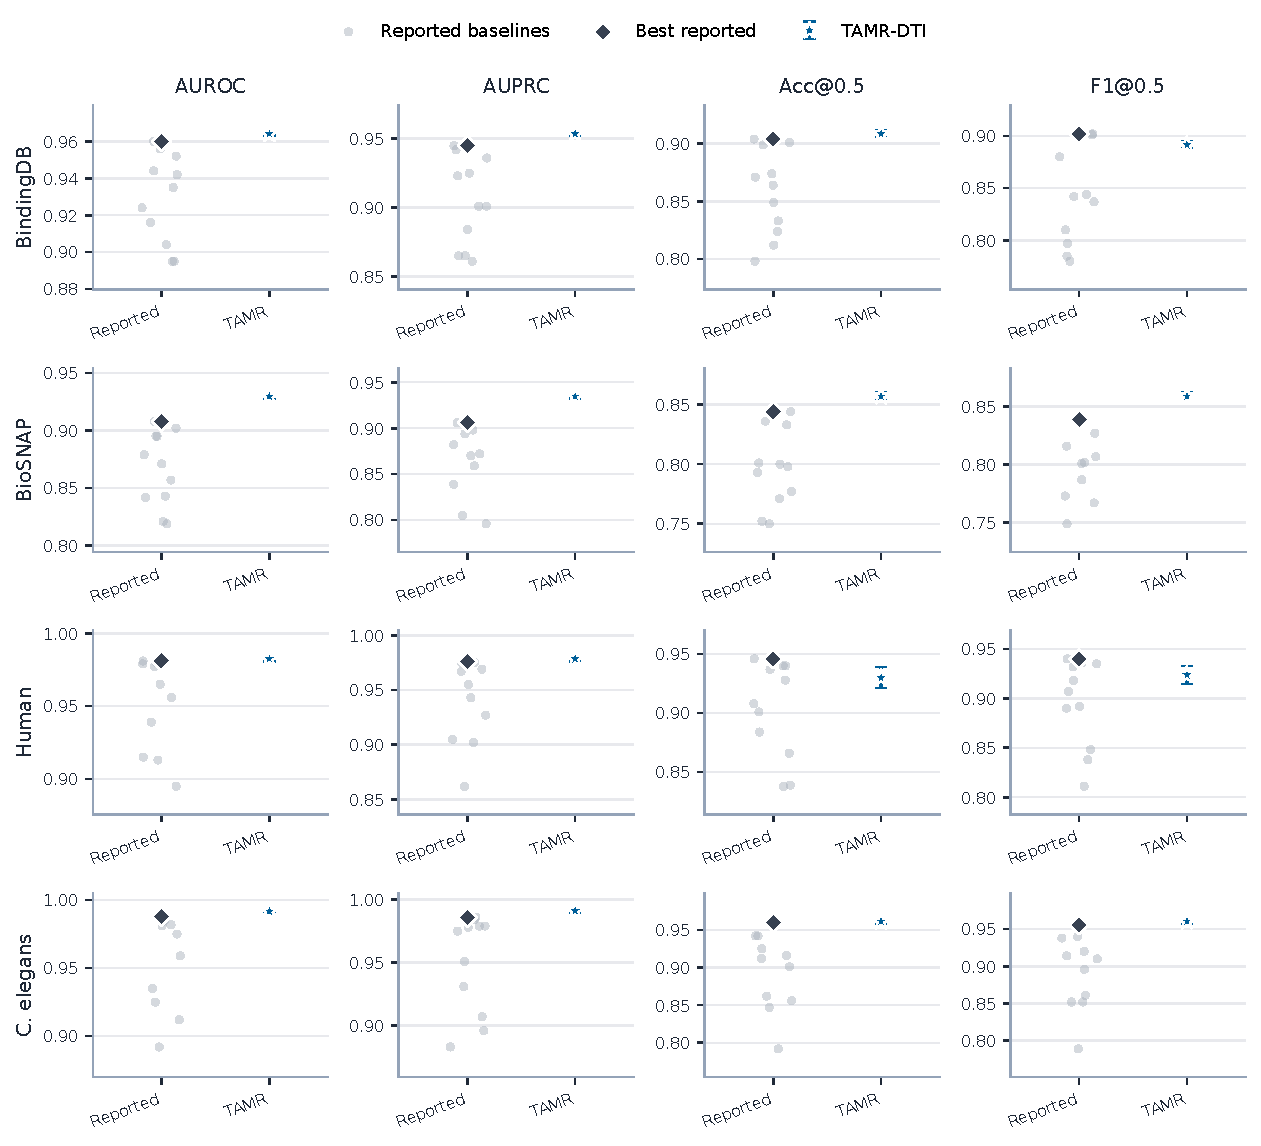
\includegraphics[width=\linewidth]{figures/main_results_comparison.pdf}
\caption{Main result comparison across four datasets and four metrics. Gray points denote reported baselines, dark diamonds denote the best reported value, and blue stars denote TAMR-DTI five-seed means with one-standard-deviation error bars. Acc@0.5 and F1@0.5 are fixed-threshold metrics.}
\label{fig:main_results_comparison}
\end{figure}

Figure~\ref{fig:all_method_ci_comparison} provides a complementary uncertainty view for AUPRC, Acc@0.5, and F1@0.5. For the reported baselines, intervals are computed from the published mean and standard deviation using the same five-run $t$-interval formula when those summaries are available; for TAMR-DTI, intervals are computed from our five seeds. This plot is again descriptive rather than paired: it shows whether the TAMR-DTI estimates sit outside or near the reported uncertainty ranges, while preserving the distinction between literature baselines and our own repeated runs.

\begin{figure}[!htbp]
\centering
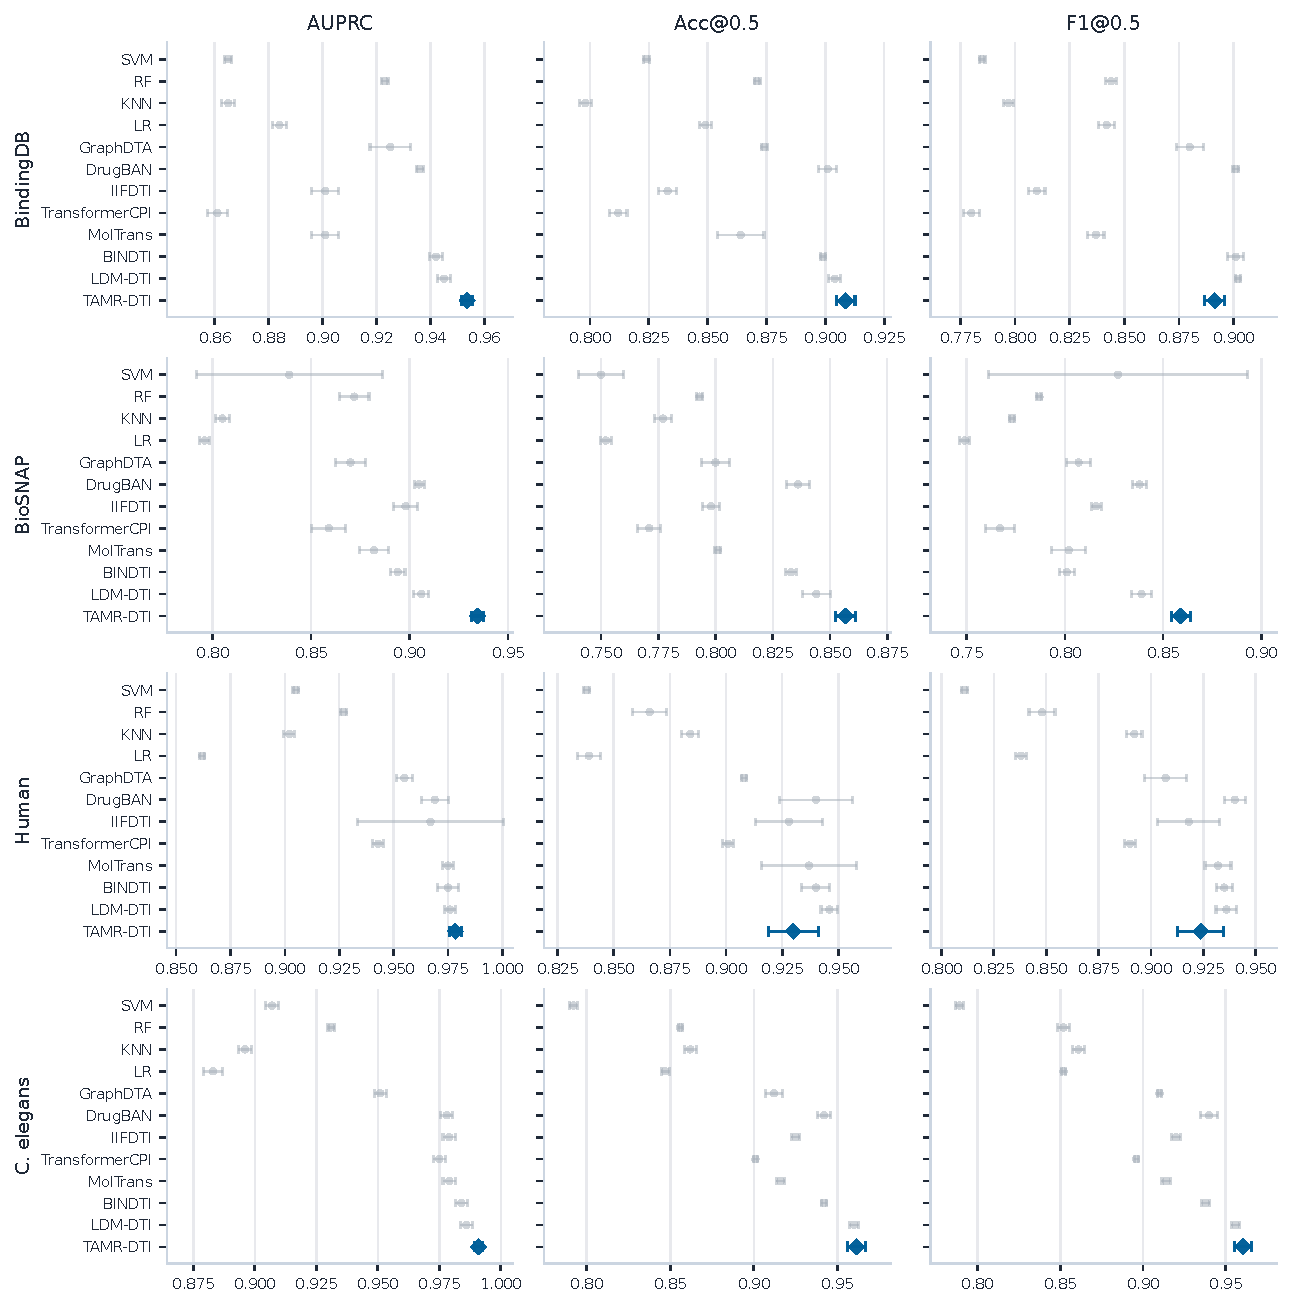
\includegraphics[width=\linewidth]{figures/all_method_ci_comparison.pdf}
\caption{All-method uncertainty comparison on AUPRC, Acc@0.5, and F1@0.5. Baseline intervals are derived from reported mean and standard deviation values, whereas TAMR-DTI intervals are computed from five local seeds.}
\label{fig:all_method_ci_comparison}
\end{figure}

The fixed-threshold results are reported in Table~\ref{tab:tamr_main_summary} and Figure~\ref{fig:main_results_comparison} for completeness, but they are secondary to the main ranking-metric claim. Acc@0.5 and F1@0.5 depend on score calibration and on the fixed threshold used for all methods, so they are more sensitive to class balance and split composition. This explains why BindingDB and C. elegans show clearer improvements in AUROC/AUPRC than in every thresholded metric, and why Human improves the ranking references while still lagging behind the strongest reported fixed-threshold scores.

\FloatBarrier
\subsection{Stability Across Seeds}

The repeated-seed analysis separates stable ranking gains from split-sensitive behavior. BindingDB, BioSNAP, and C. elegans form compact AUROC/AUPRC clusters, indicating that the ranking improvements are not driven by a single favorable seed. Human also stays above the reported-reference ranking range across most seeds, but its fixed-threshold metrics vary more strongly than the larger benchmarks. This is why the Human result is discussed as a calibration and stability limitation even though its mean AUROC and AUPRC are competitive with the strongest reported references.

The seed-level view in Figure~\ref{fig:main_seed_stability} is used for this interpretation. The plot is descriptive rather than inferential: it shows where the proposed model is stable enough to support a benchmark claim and where additional calibration and repeated-run robustness work is still needed.

\begin{figure}[!htbp]
\centering
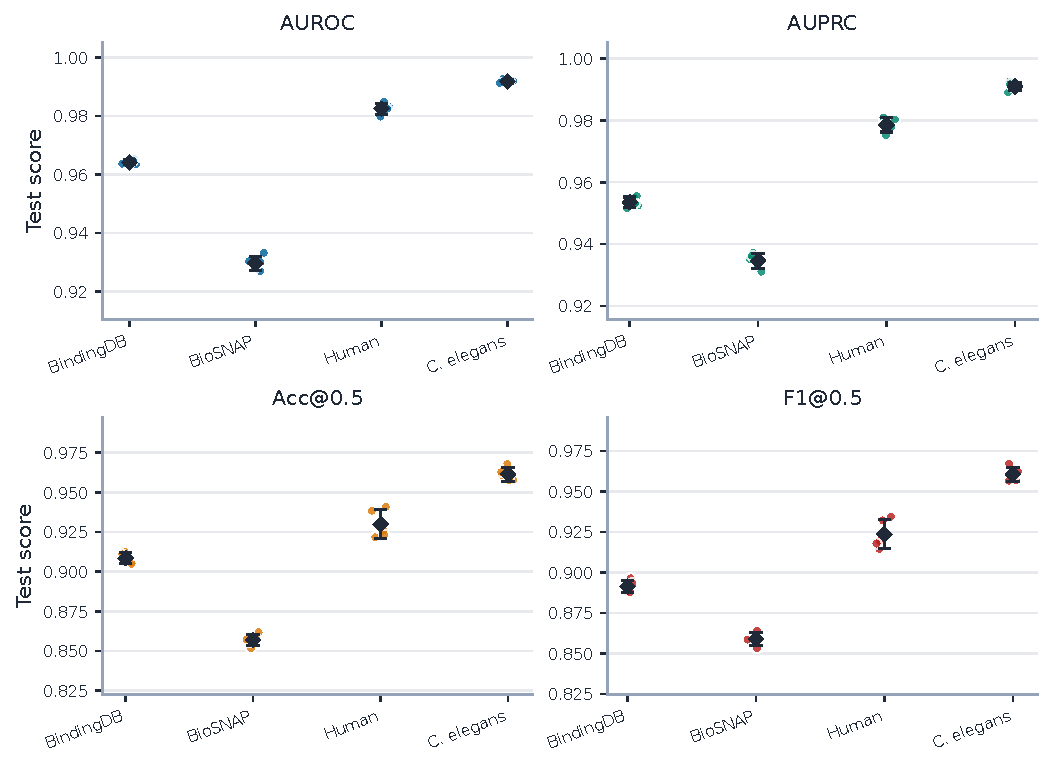
\includegraphics[width=0.92\linewidth]{figures/main_seed_stability.pdf}
\caption{Five-seed stability of TAMR-DTI on the four benchmark datasets. Dots denote individual seeds 42, 43, 44, 45, and 47; diamonds denote seed means; and error bars denote one standard deviation. Acc@0.5 and F1@0.5 use the fixed threshold 0.5.}
\label{fig:main_seed_stability}
\end{figure}

\FloatBarrier
\subsection{Ablation, Conformer Comparison, and Interpretability}

The BioSNAP gain is analyzed through the mechanism that TAMR-DTI is designed to implement rather than through separate table-by-table comparisons. The initial protein representation first conditions the selection of drug conformers, so the small-molecule geometry branch is not averaged independently of the target. The aggregated drug context then feeds back into protein encoding through FiLM modulation, protein-side Mamba refines the longer sequence-token stream, and the final bidirectional interaction module aligns the two modalities before prediction. We test this chain from three internal perspectives: module removal, conformer-count control, and model-internal evidence from conformer weights, FiLM strength, and Mamba refinement. BioSNAP is used because it is nearly balanced and gives the clearest ranking-metric improvement in the main benchmark comparison.

\subsubsection{Module ablation}

The module ablation asks whether the BioSNAP result comes from the intended cross-modal conditioning path or from a single oversized encoder. We conduct a single-seed diagnostic study with seed 42, the same train/validation/test split, the same validation-AUROC checkpoint-selection rule, and the same training configuration as the full model. Each ablated variant removes one module while keeping the remaining architecture unchanged. Because the ablation is not repeated over multiple seeds, we treat it as a diagnostic module-necessity analysis and report absolute scores rather than inferential claims. Acc@0.5 and F1@0.5 are computed at the fixed threshold 0.5.

The full model forms the upper envelope in Table~\ref{tab:biosnap_ablation}, reaching 0.933 AUROC, 0.937 AUPRC, 0.862 Acc@0.5, and 0.864 F1@0.5. The largest AUROC loss appears when target-aware conformer aggregation is removed, dropping from 0.933 to 0.916 and reducing F1@0.5 from 0.864 to 0.845. This supports the core geometry argument: conformers should not be treated as target-agnostic views, because the relevant molecular geometry depends on the protein context. Removing ligand-conditioned protein FiLM gives the largest fixed-threshold accuracy drop, from 0.862 to 0.842, which is consistent with the feedback direction in the architecture: after protein-guided conformer aggregation, the resulting drug context should still be allowed to modulate protein encoding before final interaction prediction.

\begin{table}[!htbp]
\caption{Single-seed diagnostic ablation results on BioSNAP. All variants use seed 42, the same split, validation-AUROC checkpoint selection, and fixed-threshold Acc@0.5/F1@0.5.}
\label{tab:biosnap_ablation}
\begin{center}
\scriptsize
\setlength{\tabcolsep}{4pt}
\begin{tabular}{lcccc}
\toprule
Variant & AUROC & AUPRC & Acc@0.5 & F1@0.5 \\
\midrule
Full TAMR-DTI & \best{0.933} & \best{0.937} & \best{0.862} & \best{0.864} \\
w/o Target-aware conformer & 0.916 & 0.922 & 0.844 & 0.845 \\
w/o Protein FiLM & 0.920 & 0.924 & 0.842 & 0.844 \\
w/o Protein Mamba refinement & 0.918 & 0.925 & 0.842 & 0.845 \\
w/o Bidirectional modulation & 0.920 & 0.926 & 0.848 & 0.849 \\
\bottomrule
\end{tabular}
\end{center}
\end{table}

Reading the ablation scores as drops from the full model makes the component roles clearer. The relative-drop view in Figure~\ref{fig:biosnap_ablation_drop} shows that removing the target-aware conformer module produces the largest AUROC drop, removing ligand-conditioned FiLM produces the largest Acc@0.5 drop, and removing protein Mamba refinement or bidirectional modulation yields consistent but slightly smaller degradation across the four metrics. The full model is included as the zero-drop reference, so the plot directly shows how far each ablated configuration moves from the complete TAMR-DTI setting.

\begin{figure}[!htbp]
\centering
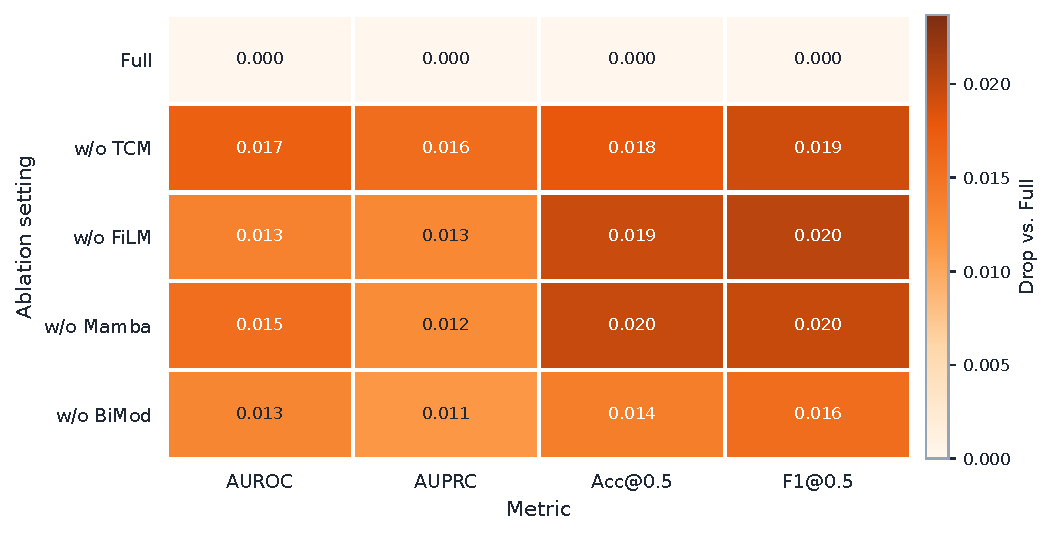
\includegraphics[width=0.92\linewidth]{figures/ablation_biosnap_seed42_drop.pdf}
\caption{Single-seed diagnostic ablation drops on BioSNAP relative to the full TAMR-DTI model. Each cell reports the relative test-score decrease caused by removing one module under the same seed, split, validation-AUROC checkpoint selection, and fixed-threshold Acc@0.5/F1@0.5; the full model is shown as the zero-drop reference.}
\label{fig:biosnap_ablation_drop}
\end{figure}

The protein Mamba and bidirectional-interaction ablations complete the same picture. Removing protein Mamba refinement lowers AUROC to 0.918 and F1@0.5 to 0.845, showing that the protein branch loses discriminative information when its token sequence is not further refined. This placement is intentional: TAMR-DTI applies Mamba to protein tokens rather than to SMILES tokens, because the drug branch is already represented through graph, pretrained, and conformer-level views, while the protein branch provides the longer sequence-token substrate where state-space refinement has a clearer role. Removing bidirectional modulation gives the smallest but still consistent degradation, with AUROC decreasing to 0.920 and F1@0.5 decreasing to 0.849. The four modules therefore act as complementary parts of one conditioning path: target-aware geometry selection, drug-to-protein FiLM feedback, protein-side sequential refinement, and final cross-modal alignment.

\subsubsection{Conformer-count comparison}

The conformer-count comparison isolates where the geometry branch helps. We compare six BioSNAP seed-42 variants that differ in the effective number of valid conformers or in the conformer aggregation rule. The $n=1$, $n=2$, and $n=4$ variants are derived from the same eight-slot conformer cache by keeping only the first $n$ valid conformer slots and masking the rest. The $n=8$ variant uses the full eight-conformer cache used in the main model, and the $n=16$ variant uses a separately generated sixteen-conformer cache to test whether a larger candidate geometry set improves the model further. Because preprocessing sorts generated conformers by computed energy, conformer count also controls the energy range exposed to the model: $n=1$ keeps only the lowest-energy conformer, $n=2$ and $n=4$ add lower-energy alternatives, $n=8$ exposes a broader geometry set, and $n=16$ adds still more candidate conformers that may also contain additional irrelevant geometry. The $n=8$ uniform-average variant keeps the same eight-conformer input but disables target-aware scoring and therefore serves as the aggregation control. All variants use the same data split, seed, optimizer, and validation-AUROC checkpoint selection; this experiment is interpreted as a conformer-count diagnostic rather than a hyperparameter search. The early-stopping patience is set to 100 epochs in this diagnostic comparison so that all variants can complete the full training horizon; Acc@0.5 and F1@0.5 are computed at the fixed threshold 0.5.

\begin{table}[!htbp]
\caption{Single-seed conformer-count comparison on BioSNAP. Conformers are energy-sorted during preprocessing; $n=1$ keeps the lowest-energy conformer only, while larger $n$ values expose additional geometries.}
\label{tab:biosnap_conformer_comparison}
\begin{center}
\scriptsize
\setlength{\tabcolsep}{3.2pt}
\resizebox{\linewidth}{!}{
\begin{tabular}{lccrrrrr}
\toprule
Variant & Effective conformers & Aggregation & Best epoch & AUROC & AUPRC & Acc@0.5 & F1@0.5 \\
\midrule
$n=1$ target-aware & 1 & Target-aware & 46 & 0.9277 & 0.9297 & 0.8578 & 0.8591 \\
$n=2$ target-aware & 2 & Target-aware & 68 & 0.9300 & 0.9322 & 0.8575 & 0.8605 \\
$n=4$ target-aware & 4 & Target-aware & 46 & 0.9297 & 0.9345 & 0.8524 & 0.8542 \\
$n=8$ target-aware & 8 & Target-aware & 51 & \best{0.9322} & \best{0.9356} & 0.8575 & 0.8624 \\
$n=16$ target-aware & 16 & Target-aware & 62 & 0.9312 & 0.9326 & \best{0.8631} & \best{0.8668} \\
$n=8$ uniform average & 8 & Uniform average & 64 & 0.9308 & 0.9340 & 0.8589 & 0.8616 \\
\bottomrule
\end{tabular}}
\end{center}
\end{table}

The results in Table~\ref{tab:biosnap_conformer_comparison} show that the eight-conformer target-aware variant gives the strongest ranking performance, reaching 0.9322 AUROC and 0.9356 AUPRC. The single-conformer variant reaches 0.9277 AUROC and 0.9297 AUPRC, which suggests that fixing the drug geometry to the lowest-energy conformer discards useful alternative spatial views. Increasing the candidate set to $n=16$ does not improve the ranking metrics over $n=8$: AUROC decreases from 0.9322 to 0.9312 and AUPRC decreases from 0.9356 to 0.9326, although fixed-threshold Acc@0.5 and F1@0.5 increase in this single-seed run. This explains why the main experiments use $K=8$: it provides the best AUROC/AUPRC tradeoff for the ranking-focused benchmark claim, while avoiding the additional geometry noise and compute cost introduced by sixteen conformers. The intermediate $n=2$ and $n=4$ variants also do not improve monotonically across all metrics, so the result should not be read as "more conformers always win." Instead, it supports a more specific interpretation: energy-sorted conformers provide a candidate geometry set, and target-aware aggregation is needed to decide which conformers are useful for a given protein.

\begin{figure}[!htbp]
\centering
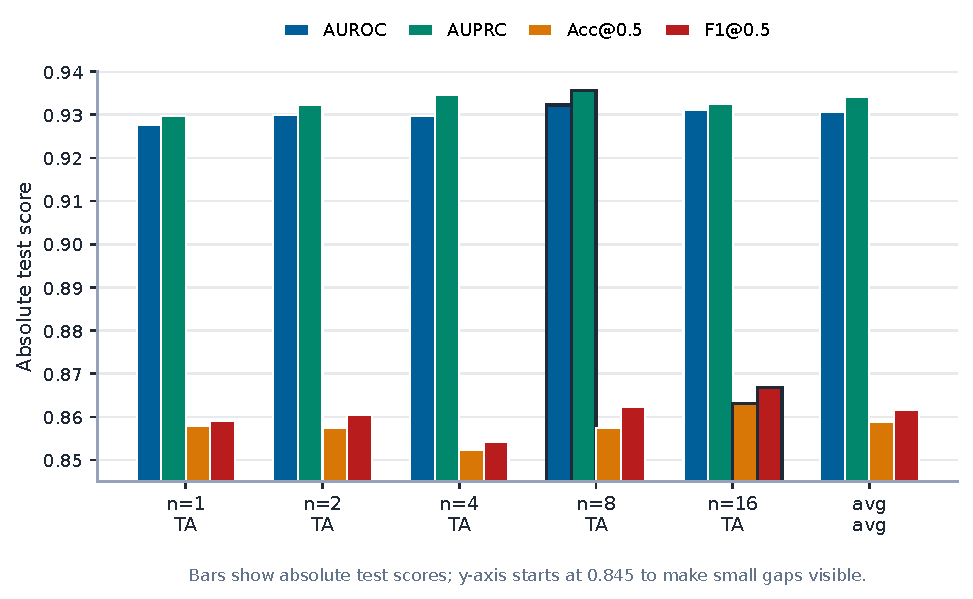
\includegraphics[width=0.82\linewidth]{figures/conformer_biosnap_seed42_comparison.pdf}
\caption{Absolute-score comparison of BioSNAP conformer-count variants, including the sixteen-conformer diagnostic run. TA denotes target-aware conformer aggregation, and avg denotes uniform averaging. The y-axis starts from 0.845 to make the small metric gaps visible; Acc@0.5 and F1@0.5 use the fixed threshold 0.5.}
\label{fig:biosnap_conformer_comparison}
\end{figure}

The absolute-score view in Figure~\ref{fig:biosnap_conformer_comparison} highlights the same tradeoff. The target-aware $n=8$ variant is highest on AUROC and AUPRC, whereas $n=16$ is higher on the fixed-threshold Acc@0.5 and F1@0.5 in this diagnostic run. We therefore interpret the conformer-count comparison conservatively: multiple conformers are useful, and protein-conditioned weighting improves ranking metrics up to the eight-conformer setting, but the fixed-threshold metrics do not support a claim that a larger conformer set dominates at every operating point.

Together with the benchmark comparison, these diagnostics explain why BioSNAP is the strongest positive case for TAMR-DTI. The gain is not attributed to a single module in isolation. It depends on protein-guided conformer selection, drug-context feedback into protein encoding, protein-side sequential refinement, and final bidirectional alignment. The conformer-count result also places the energy issue in the right scope: the lowest-energy conformer is a useful starting point, but binding prediction benefits from exposing additional geometries and letting the target representation weight them.

\FloatBarrier
\subsubsection{Interpretability analysis}

The ablation study shows that the proposed modules are useful, but it does not directly show how the full model uses them during inference. We therefore conduct a module-oriented interpretability analysis on the BioSNAP seed-42 model, using the same best checkpoint and the validation-selected threshold of 0.60 only to assign prediction groups in the diagnostic plots. The analysis covers all 5,493 BioSNAP test pairs and focuses on three quantities that are directly tied to the proposed architecture: target-aware conformer weights, ligand-conditioned FiLM modulation strength, and protein Mamba refinement magnitude. Since the protein features are pooled token representations rather than experimentally annotated residue coordinates, we interpret the visualizations as model-internal evidence instead of claiming exact biochemical binding sites.

For the target-aware conformer module, the model produces a distribution over the $K$ valid conformers of a drug molecule. For a test pair $i$, let $\mathbf{w}_i=\{w_{i1},\ldots,w_{iK}\}$ denote the conformer weights. We quantify the sharpness of conformer selection by the normalized entropy
\begin{equation}
\bar{H}_i=-\frac{1}{\log K_i}\sum_{k=1}^{K_i} w_{ik}\log(w_{ik}+\epsilon),
\end{equation}
where $K_i$ is the number of valid conformers and $\epsilon$ is a small constant for numerical stability. A smaller $\bar{H}_i$ indicates that the prediction depends more strongly on a small subset of conformers, whereas a larger value indicates softer multi-conformer aggregation.

Representative conformer-weight maps in Figure~\ref{fig:interpretability_conformer_weights} show that the model does not use a single fixed conformer pattern for all inputs. Some pairs concentrate almost all mass on one conformer, while others distribute probability over two, three, or more valid conformers. Over the full test set, the mean top-1 conformer weight is 0.241 and the mean top-1 margin is 0.069. The mean normalized conformer entropy is 0.931, indicating that the model often keeps multiple conformers active rather than forcing a hard one-hot choice. Error cases are more concentrated on average: false positives and false negatives have lower normalized entropy, 0.898 and 0.879, and higher top-1 weights, 0.267 and 0.284, respectively. This suggests that over-confident conformer selection can be one failure pattern, while correct predictions more often benefit from a softer target-aware conformer mixture.

\begin{figure}[!htbp]
\centering
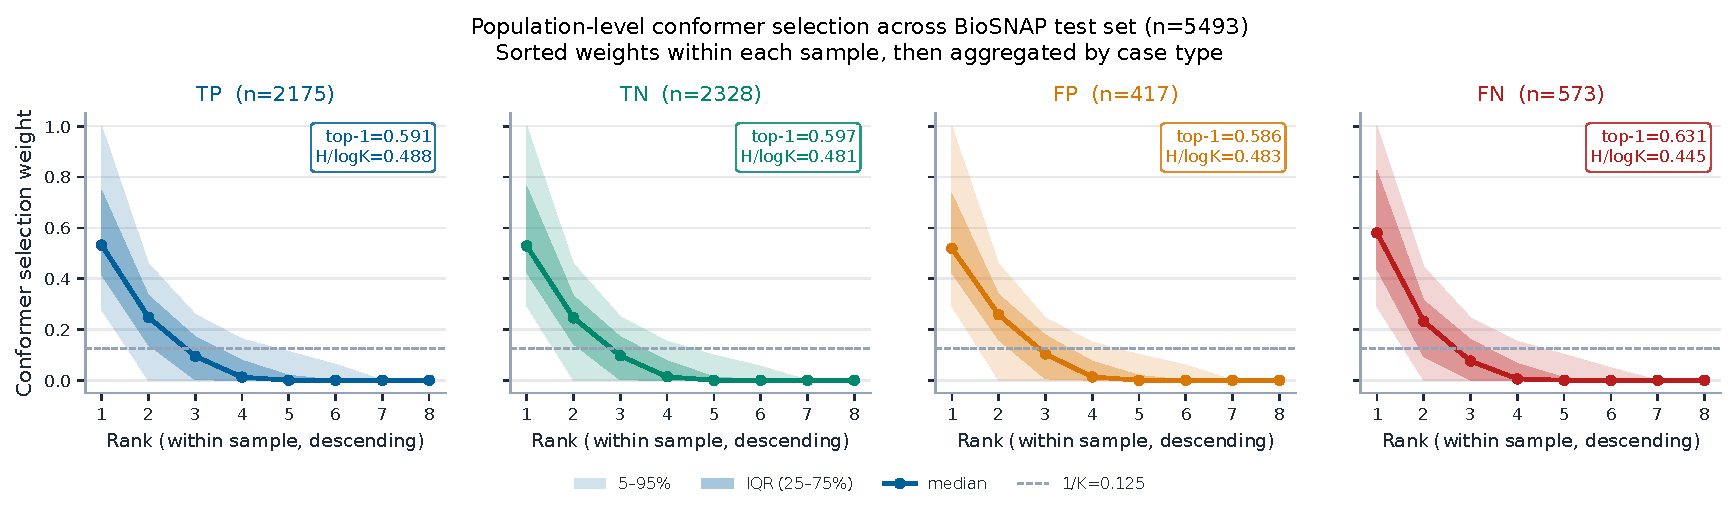
\includegraphics[width=0.92\linewidth]{figures/interpretability_conformer_weights.pdf}
\caption{Target-aware conformer-weight visualization on selected BioSNAP test cases. Rows denote representative test pairs and columns denote the eight conformer slots. Color intensity indicates the conformer selection weight assigned by TAMR-DTI.}
\label{fig:interpretability_conformer_weights}
\end{figure}

We next inspect the ligand-conditioned protein modulation module. In TAMR-DTI, the drug context controls FiLM parameters in the protein encoder, so the protein representation is updated as
\begin{equation}
\widetilde{\mathbf{H}}_{p}^{(l)}
=\mathbf{H}_{p}^{(l)}\odot(1+\boldsymbol{\gamma}_{d}^{(l)})
+\boldsymbol{\beta}_{d}^{(l)},
\end{equation}
where $\boldsymbol{\gamma}_{d}^{(l)}$ and $\boldsymbol{\beta}_{d}^{(l)}$ are generated from the drug-side context at protein layer $l$. We measure the layer-wise modulation strength as
\begin{equation}
M_l=\|\boldsymbol{\gamma}_{d}^{(l)}\|_2+\|\boldsymbol{\beta}_{d}^{(l)}\|_2.
\end{equation}
The FiLM statistics in the right panel of Figure~\ref{fig:interpretability_module_statistics} show that the drug-to-protein feedback signal is not negligible. The first protein encoding layer has the strongest average modulation, with $M_1=0.0263$, followed by $M_2=0.0160$ and $M_3=0.0166$. This pattern is consistent with the design goal of TAMR-DTI: drug-side information is injected early enough to condition protein feature extraction, and subsequent layers further transform the conditioned representation instead of treating the protein as a fixed static embedding.

For the protein Mamba refinement module, we compare the protein tokens before and after the Mamba block. Let $\mathbf{h}_t$ be the input token at protein position $t$, $\mathbf{h}^{M}_t$ be the corresponding Mamba-refined token, and $g=\sigma(\alpha)$ be the learned residual gate. We compute the gated refinement magnitude
\begin{equation}
R_t=g\|\mathbf{h}^{M}_t-\mathbf{h}_t\|_2.
\end{equation}
The learned gate is 0.129 in the BioSNAP checkpoint, which means that the model does not overwrite the protein encoder representation, but adds a controlled Mamba-based residual. Across the full test set, the mean gated refinement magnitude is 0.121 and the mean maximum token-level refinement is 0.124. The middle panel of Figure~\ref{fig:interpretability_module_statistics} compares this statistic across true positives, true negatives, false positives, and false negatives; the values are close but not identical across groups, indicating that the Mamba branch acts as a stable sequence-refinement component rather than an unstable classifier shortcut.

\begin{figure}[!htbp]
\centering
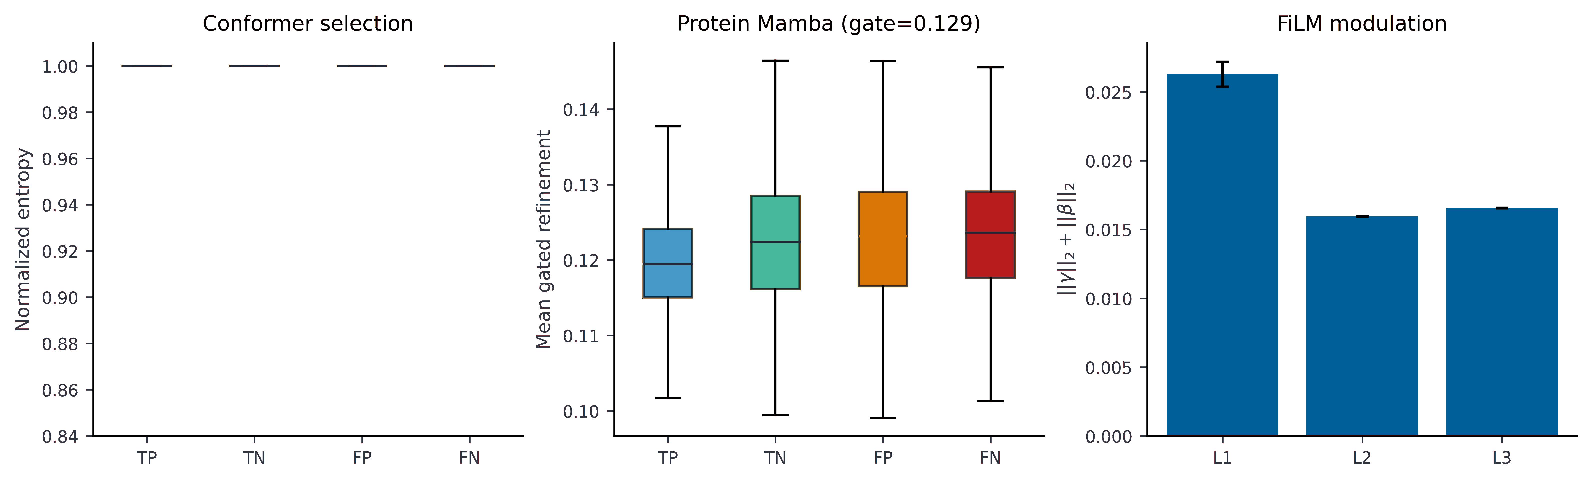
\includegraphics[width=0.95\linewidth]{figures/interpretability_module_statistics.pdf}
\caption{Module-level interpretability statistics on the BioSNAP test set. The conformer panel reports normalized conformer-weight entropy across prediction groups; the protein Mamba panel reports gated token-refinement magnitude; and the FiLM panel reports layer-wise ligand-conditioned modulation strength.}
\label{fig:interpretability_module_statistics}
\end{figure}

The token-level heatmap in Figure~\ref{fig:interpretability_mamba_refinement} further visualizes $R_t$ along the 128 protein token positions for selected representative cases. The refinement is not uniformly distributed across all protein tokens. Instead, different drug-target pairs show different local peaks, which indicates that the Mamba block adjusts the protein representation in a sequence-position-dependent manner. This complements the ablation result in Table~\ref{tab:biosnap_ablation}: removing protein Mamba refinement reduces BioSNAP performance, and the interpretability analysis shows that the retained module contributes a controlled, non-uniform refinement signal during inference.

\begin{figure}[!htbp]
\centering
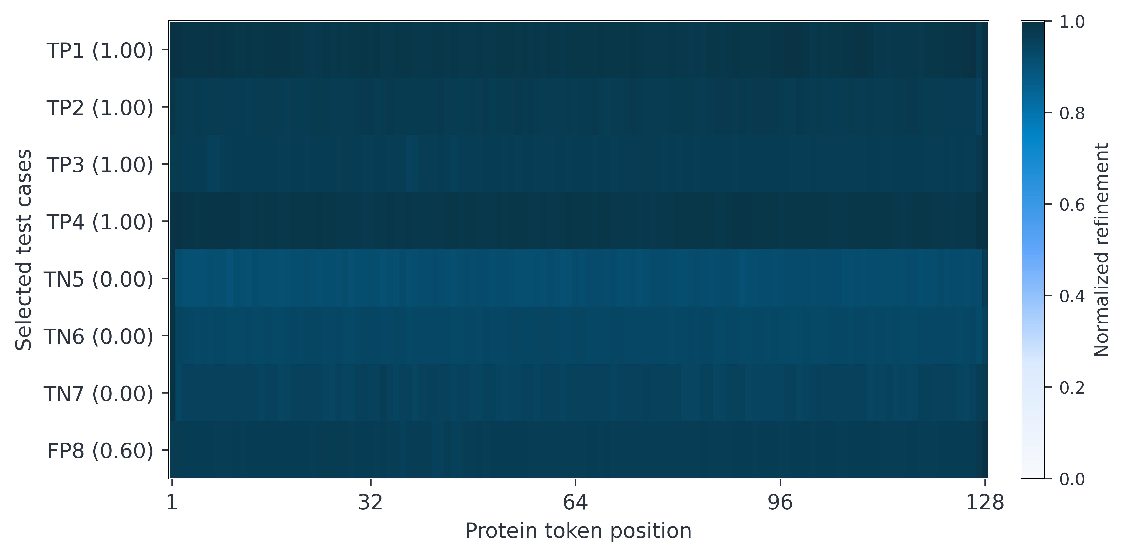
\includegraphics[width=0.92\linewidth]{figures/interpretability_mamba_refinement.pdf}
\caption{Protein Mamba refinement heatmap for selected BioSNAP test cases. Each row corresponds to a representative drug-target pair, the horizontal axis denotes pooled protein token positions, and color intensity denotes normalized gated refinement magnitude.}
\label{fig:interpretability_mamba_refinement}
\end{figure}

Overall, the interpretability results support the same conclusion as the ablation analysis from a different angle. Target-aware conformer aggregation exposes sample-specific conformer usage; FiLM confirms that protein encoding is conditioned by the drug context; and Mamba refinement provides a gated, token-dependent update to the protein sequence representation. These observations make the BioSNAP improvement more interpretable: TAMR-DTI does not rely only on a larger multimodal encoder, but uses explicit mechanisms to coordinate drug geometry, ligand-conditioned protein encoding, and sequential protein refinement before final interaction prediction.

\FloatBarrier
\clearpage
